% % % % % % % % % % % % % % % % % % % % % % % % % % % % % % % %
% This package was originally developed by Professor Arthur   %
% Baragar. It was updated in 2016 by Professor Rebecca Gill.  %
% For more information on this revised template, contact Dr.  %
% Gill at rebecca.gill@unlv.edu. See below for revisions.     %
% The content in the sample chapters was contributed by both  %
% Baragar and Dr. Gill. Additional content explaining the     %
% current (as of June 2016) UNLV Graduate College formatting  %
% requirements is taken directly from the September 17, 2015  %
% "Organization of the Thesis and Dissertation Compiled       %
% Manuals."                                                   % 
% % % % % % % % % % % % % % % % % % % % % % % % % % % % % % % %

% % % % % % % % % % % % % % % % % % % % % % % % % % % % % % % %
%                R E V I S I O N   H I S T O R Y              %
%                                                             %
% 6/29/2016: Updates to language in the sample chapters.      %
%	     Extended discussion of how to organize the       %
%	     bibliography using natbib. Replaced original CV  %
%            page with a CV template using the article class. %
% 6/21/2016: Overhaul of the original Baragar template to     %
%            meet UNLV Graduate College requirements as per   %
%            the September 17, 2015 "Organization of the      %
%            Thesis and Dissertation Compiled Manuals" here   %
%            www.unlv.edu/sites/default/files/page_files/27/  %
%            GradCollege-ThesisDissertation-Manual.pdf        %
% % % % % % % % % % % % % % % % % % % % % % % % % % % % % % % %

\documentclass[oneside,12pt]{book}
% The option oneside is required for UNLV theses.
% Font can be 11 or 12 point only
\usepackage{amsthm,amssymb,amsmath,latexsym,graphicx} 
% Optional packages.
\usepackage{setspace,UNLVthesis} 
% Required packages.  
\usepackage[round]{natbib}
% This loads the natbib package, which is a powerful bibliography formatting system.
\bibpunct[, ]{(}{)}{;}{a}{}{,}
% This command sets the formatting of the citations. Adjust as needed for your style.
\usepackage{url}
\urlstyle{same}
% The URL package is used to format the URLs in the document. This way, you don't have to "escape" the characters that appear in the URL. You'll just type \url{www.myurl.com}. The second command makes sure that they appear in the same font as the rest of the document.
\usepackage{pdfpages}
\usepackage{booktabs, caption}	
% This package formats the tables correctly.
\usepackage{rotating}
%\usepackage{float}
\pagestyle{unlv} 
% This is defined in UNLVthesis.sty. 
\setlength{\footskip}{40pt}
\usepackage{longtable}
\usepackage{tablefootnote}
% Allows me to add footnotes to tables.
\usepackage{threeparttable}
\usepackage[english]{babel} 
% This is for the dummy text in the chapters. You won't need this.
\usepackage{dcolumn}
\usepackage{adjustbox}
\usepackage{blindtext}
\usepackage{amssymb}
% This is also for demonstration purposes only. You should remove all commands related to this package when you insert your own text. They all begin with \blind or \Blind.
\usepackage{rotating, floatpag, fancyhdr}
\usepackage[capitalise, noabbrev]{cleveref}
% This package lets you use the \cref command to make cross references. Don't load packages after this one; this one needs to go in last.

\newtheorem{theorem}{Theorem}
\newtheorem{corollary}[theorem]{Corollary}  
\newtheorem{lemma}[theorem]{Lemma}
% These define the format and numbering of theorem like environments. Corollaries and Lemmas are numbered as theorems. These may be commented out when theorems are not used.


\theoremstyle{definition}
\newtheorem{definition}{Definition}
\newtheorem*{introduction}{Introduction}
\newtheorem*{conclusion}{Conclusion}
% This environment is not in italics, like theorems are.These define the format and numbering of definition like environments. The * means it is unnumbered. Again, these can be commented out when theorems are not used

% Put definitions here.  
	
	% This creates the page style for a landscape page
	\fancypagestyle{floatpage}{
		\fancyhf{}
		\renewcommand{\headrulewidth}{0pt}
		\fancyfoot[C]{\makebox[\textwidth][r]{
				\smash{\raisebox{\dimexpr\footskip+.5\textheight}{\rotatebox{90}{\thepage}}}}}
	}
	
	% This creates a page style for a portrait page
	\fancypagestyle{plain}{
		\fancyhf{}
		\renewcommand{\headrulewidth}{0pt}
		\fancyfoot[C]{\thepage}
	}
	
\begin{document}

\pagenumbering{roman}
	% Items before Chapter 1 have roman numbers (if any).
\thispagestyle{empty}%This page has no page number.

\begin{center}
 THE TITLE OF YOUR THESIS OR DISSERTATION\\*[36pt]
	 % The title can be no more than 80 characters -- UNLV rule. If it spans more than one line, it is single spaced and wrapped in an inverted triangle shape. Use \\ for a manual line break if necessary.
	 %  The command \\*[Xpt] means carriage return with a Xpt gap.  These numbers can be adjusted to improve the look.
	 % Do not use hyphens to divide words at the end of lines.
	 % The title must be in all capital letters.

\normalsize By\\*[36pt]

 Your Legal Name\\*[32pt] 
	 % This is your legal name as recorded in MyUNLV

 Bachelor of Arts -- Political Science\\*[-12pt] 
 University of Alberta, Canada\\*[-12pt]
 1986\\*[36pt]
	% This is a degree you already have
 A thesis submitted in partial fulfillment\\*[-12pt]
 of the requirements for the\\*[32pt]

 Doctor of Philosophy -- Political Science\\*[36pt]
 
 Department of Political Science\\*[-12pt]
 College of Liberal Arts \\*[-12pt]
 The Graduate College\\*[32pt]

 University of Nevada, Las Vegas\\*[-12pt]
 May 2017
\end{center}
 
	% Replace this file name with the name of your title page.
\thispagestyle{empty}

\begin{center}
	\vspace*{\fill}
	Copyright 2017 by Your Legal Name\\
	All Rights Reserved	
	\vspace*{\fill}
\end{center}

% From the 9/1/2015 UNLV Graduate College: General Guidelines for Theses and Dissertations:
% * The thesis or dissertation author automatically owns copyright to the document since it represents the author's original documented work.
% * If applicable, the copyright page is inserted after the title page in the document. Remember, this page is optional unless you register with the United States Copyright Office. Then you must have the copyright page. ...
% * If submitting in December, date for January of the following year.
% * Students have the opportunity to register a copyright on their thesis or dissertation with the U.S. Copyright Office through ProQuest. This is strictly optional, and there is a fee associated with the service. This fee is paid directly on the ProQuest site at the time of electronic submission.
% * More Information on Copyright is available at the U.S. Copyright Office’s website: http://lcweb.loc.gov/copyright.
% * Answers to frequently asked copyright questions can be found at http://www.copyright.gov/help/faq/. 
	% A copyright statement is optional, but recommended. Rename.
    % The copyright page has no page number -- the title page is always page i and the
   % Thesis Approval page is always page ii. The Graduate College inserts this for you.
\newpage \setcounter{page}{3}

\chapter*{ABSTRACT}
\addcontentsline{toc}{schapter}{Abstract}% This command adds the Abstract to the table of contents.

\begin{center}
\textbf{THE TITLE OF YOUR THESIS OR DISSERTATION}

By

Your Legal Name

 Dr.\ My Chair, Dissertation Committee
 Chair\\*[-12pt]%Single spaced.
 Professor of Political Science \\*[-12pt]
 University of Nevada, Las Vegas  %
 \end{center}

The abstract would be here.  The purpose of this package is to give some advice about using \LaTeX\ to prepare their thesis, and to illustrate, via an example (this document), what the package produces, as well as provide a template.  This package should be used in conjunction with the source files. It must be numbered iii and be double spaced. All other formatting must be per the requirements of disciplines style guide or style guide that the thesis or dissertation committee members agreed upon.
 
	% This is where the abstract goes. Rename. 
\chapter*{ACKNOWLEDGMENTS}
%\addcontentsline{toc}{schapter}{Acknowledgments}

I would like to thank Dr.\ Baragar for making this template and Dr.\ Gill for updating it. 

This page is optional. However, Dr.\ Gill recommends that you include this section and give it some significant thought. 


  
	% This is optional. Rename.
\chapter*{Dedication}

To Mom. 
	% This is also optional. Rename.
	% You could add a preface here if you want. See the formatting guide.

%%% TESTING TOCLOFT
%\cleardoublepage
%\tableofcontents
%\cleardoublepage
%\addtocontents{lof}{\lofheading}% add heading to the first page in LoF
%\listoffigures
%\cleardoublepage
%\addtocontents{lot}{\lotheading}% add heading to the first page in LoT
%\listoftables
%\cleardoublepage
%
%\mainmatter
%\addtocontents{toc}{\tocheading}% add heading to the first page in ToC, after frontmatter entries
%
%\mainmatterchaptoc% activation of chapter entries formatting in the mainmatter
%%%

\renewcommand\contentsname{Table of Contents} 
	% This adjusts the way the Table of Contents label looks.
\tableofcontents 
	% This inserts table of contents. Use headings and subheadings consistently in your chapters and they will appear properly here. See the note in SampleChapter1 about how to use the square brackets as a hack to get the colon to appear between the chapter number and the chapter title. 
\listoftables \addcontentsline{toc}{schapter}{\listtablename}
	% Comment out if there are no tables. If you use an appendix, be sure to label these with the appropriate table notations. Tables in the appendices need to appear in this list.
\listoffigures \addcontentsline{toc}{schapter}{\listfigurename}
	% Comment out if there are no figures. If you use an appendix, be sure to label these with the appropriate figure notations. Figures in the appendices need to appear in this list.



\newpage 
	% This sets the page numbers properly.
	
\pagenumbering{arabic} 
	% Chapter 1 begins on page 1.

\chapter[: Introduction]{Introduction} 
% The title in the square brackets is a workaround to get the colon and space to appear properly in the table of contents. Just include a colon, a space, and then the title of your chapter in the square brackets. The title should appear without the colon and space in the curly brackets.

This section of the template will give you some information about the basic formatting requirements for your thesis or dissertation. To the extent possible, these requirements have been built into this template. The text below comes directly from the ``UNLV Graduate College: General Guidelines for Theses \& Dissertations'' September 1, 2015, update (\url{https://www.unlv.edu/sites/default/files/page_files/27/GradCollege-ThesisDissertation-Guidelines.pdf}) and the ``UNLV Graduate College's Organization of the Thesis and Dissertation Compiled Manuals'' updated September 17, 2015 (\url{https://www.unlv.edu/sites/default/files/page_files/27/GradCollege-ThesisDissertation-Manual.pdf}). It is your responsibility to check with the Graduate College to confirm that there have been no subsequent updates to the formatting requirements. If you see that there are changes that impact this template, please contact Dr.\ Gill at \url{rebecca.gill@unlv.edu}. 

\section{Fonts}

The font must be a standard style that is clear and readable, typically in 11, or 12 point size. Do not use cursive, script or italicized fonts except where allowed or required by your chosen style guide (Chicago, APA, ASA, MLA, etc.). Font size must be consistent throughout the text. Chapter titles and section titles can be larger font size than the standard text, if in accordance with the student's approved style guide and advisory committee. This style decision must be applied consistently throughout the text. The font size of tables and figures can be smaller than the standard text if in accordance with the student's style guide and advisory committee (8 pt.\ minimum). This style decision must be applied consistently throughout the text.

You can find an instruction manual on how to create this page on the Thesis and Dissertation
website. 

\section{Spacing and Margins}

 The document must be double spaced; the only exceptions are captions, foot‐ notes, long  quotations, bibliographic references, table titles and descriptions, figure titles and descriptions,  inserted materials such as tables, images, diagrams, graphs, etc., and the author's curriculum  vit\ae. Extended direct quotations must be handled according to the rules of your chosen style guide and the direction of your advisory committee. 
 
 Paragraphs should be indented the same number of spaces throughout the document, and
 spacing between paragraphs should be consistent. Spacing around titles, headings and subheadings should be consistent and match the student's chosen style guide. You can find an instruction manual on how to create this page on the Thesis and Dissertation website. 

 All pages should have a 1” margin on all sides (top, bottom, right, and left). Top and bottom margins must be blank with the exception of the page number at the bottom center of the page (please see item 2 – Page Numbering). Do not include other headers or footers. You can find an instruction manual on how to create this page on the Thesis and Dissertation website. 

 
	% Replace these with your chapters. Rename these as necessary.
\chapter[: Where Do I Get \LaTeX?]{Where Do I Get \LaTeX?}

\LaTeX\ is a freeware application.  It was originally designed by Donald Knuth at Stanford, and is being maintained by the (mostly European) academic community.  There are versions that run on PC, Mac, and Linnux systems, among others.  Though the compilers are platform dependent, the source files are not. 

\section{Getting \LaTeX Up and Running}

A great place to start is the \LaTeX-project website site about obtaining \LaTeX\. It is here: \url{https://latex-project.org/ftp.html}. The way you proceed is usually going to involve installing a version of \LaTeX\ and then installing an editor.

\section{Getting your \TeX\ distribution}

You will need to install your \TeX\ distribution before you try to install an editor. For most beginning users, you'll want to install using the default options. The original PC version of \LaTeX\ is MikTeX.  It can be obtained from \url{www.miktex.org}. You can also try proTeXt, which is a \TeX\ distribution for Windows that is based on MikTeX and adds a few extra features. You can find this here: \url{http://www.tug.org/protext}.

The \TeX\ distribution for Mac OS is called MacTeX. It can be downloaded here: \url{http://www.tug.org/mactex/}. If you're using Linux, you probably already have a TeX system installed. If you don't, you should install TeX Live from here: \url{http://www.tug.org/texlive}.

\section{Choosing and installing an editor}

 Then, you'll probably want to choose \LaTeX\ editor. Although MikTex and MacTex both come with front ends, there are heaps of very good open source (free!) editors from which to choose. Dr.\ Gill prefers TeXstudio, which is free from \url{http://texstudio.sourceforge.net}. This editor supports Windows, Mac OS, and Linux. TeXworks (\url{https://www.tug.org/texworks}) and TeXmaker (\url{http://www.xm1math.net/texmaker}) are also very good, and they work on all of the major operating systems. Dr.\ Baragar prefers Winedt (\url{http://www.winedt.com}), which works on Windows. 
 
 Sometimes, you might want to make some edits on the fly. For this, you might want to use an online, web-based editor. For this, my favorite is ShareLaTeX. It has a free version and a subscription version. However, if you share ShareLaTeX with others, you can unlock the premium features for free! So, if you get ShareLaTeX from this link, you'll help me unlock free Dropbox integration! \url{https://www.sharelatex.com?r=8c76f322&rm=d&rs=b}. Other good online editors are Overleaf \url{https://www.overleaf.com} and Authorea \url{https://www.authorea.com}, both of which also have free versions and paid subscription-based versions.
 
 Of course, things are always changing in the world of \LaTeX\ . Dr.\ Gill compiled this list as of 2016, but there may be even better options available to you now. Be sure to search for something like ``Best \LaTeX\ Editors 20XX'' (where the 20XX is the current year) to see if you can find something new.
 
\section{Getting started}

It's probably best to extract these files into a new folder for your thesis or dissertation. You should keep a copy of the originals, though, in case you accidentally change something that sends the entire thing down a spiral of warnings, errors, and failed rendering. If your dissertation is temporarily called ``Project X,'' you would extract all of these into a folder of that name.

From there, you'll edit the content in the main files. You might want to change the names of the chapter files. If you do, be sure to change the names in the $\backslash include\{SampleChapterX\}$ entry in the UNLVthesisTemplate.tex file. You're probably going to need more than three chapters, so you'll need to create more and then add $\backslash include\{SampleChapterX\}$ entries in the UNLVthesisTemplate.tex file. 

You will also probably (hopefully!) need a bibliography. Dr.\ Gill has formatted this template to use \texttt{natbib}, which is my favorite. You might want to do this differently, depending upon which formatting style you need to use for your works cited list. Natbib is very flexible (especially for author-date formats). You can find more information on customizing your bibliography using natbib by consulting the Reference Sheet on CTAN's natbib page: \url{http://mirrors.ctan.org/macros/latex/contrib/natbib/natnotes.pdf}.

\section{Resources}

Probably the best place to start is on the starter page for the website \url{www.ctan.org/starter}. This includes links to {\it The (Not so) short introduction to
\LaTeX2$\epsilon$}, by Tobias Oiteker, et al.\ It is a 110 page free
document \citep{oetiker2015notsoshort}. You'll also want to bookmark the \LaTeX\ Wikibook: \url{https://en.wikibooks.org/wiki/LaTeX}. The nice thing about this resource is that it is updated regularly with new information. There are also countless tutorials and videos on the internet. Google is your friend!

There are several books out there that might also be helpful. Some of the old favorites might work, and they might help you avoid having to use a lot of the newer packages. The downside is that these books are out of date about these new packages, so you might miss out on a very simple way to do what you need to do. With that caveat, here are some of the classics courtesy of Dr.\ Baragar: One perennial favorite is {\it The \LaTeX\ Companion} by \citet{goossens1994latex}, but this is probably more for an expert. {\it A document preparation system \LaTeX} by \citet{lamport1986document} is more suited to the beginner. There is also {\it A guide to \LaTeX}, by \citet{kopka2004guide}, but Dr.\ Baragar thinks this, too, is for the expert. 

Because of the rapidly evolving nature of open source programming languages, you may prefer to use the online guides and discussions at places like the \TeX\ section of StackExchange (\url{http://tex.stackexchange.com/questions/ask}). Search first and familiarize yourself with the protocol before you ask a question; the folks over there get irritated if you ask a duplicate question or fail to provide a minimal working example (MWE)!


\chapter[: A Sample Document]{Going Beyond the Text}

One of the more difficult formatting challenges you'll have is dealing with the various special features that many dissertations and theses require. You're likely to need tables, figures, equations, algorithms, or other non-prose representations of your work. Below are some examples of how to accomplish this.

First, a couple of notes from the Graduate College. This is taken directly from the formatting guidelines. This template will accomplish most of this automatically, provided that you use the labeling templates you'll find in this chapter. The first level content below is from the Graduate College, and my commentary for each appears in the second level content.

\begin{itemize}
	\item Be sure that all inserted information (images, tables, graphs, diagrams, etc.) are labeled with a title and number (Example: Table 1. Total Graduate Students from 1986 to 1997). If applicable, the label listed in the text must match the label listed in the List of Tables or List of Figures exactly. The numbering must be consecutive, per the requirements of your style.
		\begin{itemize}
			\item This will happen automatically, provided that you use the proper environments and label tags. The examples are below. 
		\end{itemize}
	\item If a table or a figure is landscape oriented, the table's/figure's label must be landscaped oriented to match.
		\begin{itemize}
			\item There is an example of this below in \cref{fig:fig2} on \cpageref{fig:fig2}. 
		\end{itemize}
	\item If you have 5 or more of an embedded item (tables, figures, equations, algorithms, etc.), the must be referenced in a list in the front of your document. The list should be titled ``List of...,'' so tables would be ``List of Tables,''  figures would be ``List of Figures,'' etc. If you 4 or fewer of an item, it does not need to appear in a list. 
		\begin{itemize}
			\item This is already automated in this template \textit{except} for lists of equations or theorems. To do this, you would need to use the \textsf{tocloft} package. This would require completely rewriting the \texttt{UNLVthesisTemplate.tex} and \texttt{UNLVthesis.sty} files. Dr.\ Gill hopes to undertake this formatting overhaul in an upcoming version of the template.
		\end{itemize}	
	\item Tables and figures must be clearly delineated from the text. This can be done by line breaks, (a double space), borders, or a delineation that is approved by your style guide. The title and description of tables, figures, images, etc. are considered to be part of the table, figure, or image and must be clearly delineated from the text as well.
		\begin{itemize}
			\item This is automated in the template. You can also use the placement operators and (if you must) vertical or horizontal spacing adjustments to get the look you want. 
		\end{itemize}
	\item Images, tables, diagrams, graphs, etc. embedded into your document must fit on a single page. You can use a smaller font size on tables, figures, and other inserted materials. If a table does not fit within your text on a single page it must be moved to an appendix. You can either give	each table its own appendix or you can create a single appendix containing multiple tables.
		\begin{itemize}
			\item If you have a table that spans more than one page, it has to go in an appendix. You will probably want to use the \textsf{longtable} package to accomplish that. 
		\end{itemize}

\end{itemize} 

\section{Equations, Algorithms, and Theorems}

In the current version of this template, there is no support for a table of equations. If you have more than five numbered equations in your thesis or dissertation, you are required to include a table of equations. In order to do this, you will probably have to use the \textsf{tocloft} package. If you do that, you'll basically need to rewrite much of the \texttt{UNLVthesisTemplate.tex} and \texttt{UNLVthesis.sty} documents. Dr.\ Gill is currently working on incorporating the \textsf{tocloft} package into a future version of this template.

To type an equation in the line, put it between dollar signs.  For
example, $y = \beta_0 + \beta_1 X_1 + \varepsilon$.  If you would like to highlight that equation without numbering it, you can use this notation:  $$y = \beta_0 + \beta_1 X_1 + \varepsilon$$
If the equation is to be referenced, then do the following:
\begin{equation}\label{eq:Equation1}
	%This is the label of the equation -- LaTeX will number it.
	y = \beta_0 + \beta_1 X_1 + \varepsilon
\end{equation}

Note that, if you have five or more numbered equations in your thesis or dissertation, you'll need to include a Table of Equations. You can then reference the equation (\cref{eq:Equation1}) has no
non-trivial solutions in the integers. 

Some results are important, and you may wish to express them as a theorem.

\begin{theorem}[Fermat's Last Theorem]\label{theorem 1}  The equation $x^n+y^n=z^n$ has no solutions $x,y,z\in \mathbb Z$ for $n\geq 3$ and $xyz\neq 0$.
\end{theorem}

You can then reference the theorem using the \textsf{cleveref} package. \Cref{theorem 1} was proved by Wiles.  The proof does not appear in \citet{kopka2004guide}.

Sometimes you might want to have aligned equations, like the following:
\begin{align} %\label{eq:Equations} put the label here to label both, removing individual labels
	\frac{\partial\hat{Y}}{\partial X_1} &= B_1 \label{eq:Equation2} \\
	\frac{\partial\hat{Y}}{\partial X_2} &= B_2 \label{eq:Equation3}
\end{align}

You could also choose to place the label directly after the align command, which would label the pair of equations instead of labeling each of the equations separately. 

\section{Figures and Tables}

You will probably need to use figures or tables in your dissertation or thesis. Below are a few examples here so that you can see how to do this properly. Remember to label these figures and tables so that they appear properly in your list of tables and/or list of figures.

A picture is shown in  \cref{fig:fig1}.
\begin{figure}[h]
		%This [h] tells LaTeX to try to put the picture here. Without it, it will go to the top of the next page. There are a number of other placement operators that can help you achieve the look that you want.
\begin{center}
{\mbox{
\includegraphics[height=140pt]{fig1.png}}}
\end{center}
\caption{\label{fig:fig1}This is a Figure 1 Figure}
\end{figure}
	% Be careful with empty lines -- remember, they mean new paragraph.
    % There are no empty lines before and after the figure environment since
    % I do not want a new paragraph here.

Now, let's try to include a landscape image. This is required for images (or tables) that are too wide to fit on a single page. Obviously, \LaTeX\ is going to put this where it will fit, so you'll have to look to \cpageref{fig:fig2} to find \cref{fig:fig2}.

\begin{sidewaysfigure}
	\begin{center}
		
\includegraphics[scale = .5]{huge-placeholder.png}
\end{center}
\caption{\label{fig:fig2}This is a Landscape Figure}
\end{sidewaysfigure}

You can use all sorts of different programs to create graphics.\footnote{Dr.\ Gill likes using \textsf{R} to make cool data visualizations!} Usually, .png files seem to work best in \LaTeX\ . If your graphics are in a different format, you can just open the image in my default ``paint'' program and save the image as a .png file. 

You might also want to include a table. Your \LaTeX\ editor might include a wizard for creating tables easily. Dr.\ Gill actually likes to use an online table editor from the Tables Generator website: \url{http://www.tablesgenerator.com/}. Be sure to put your table in the tabular environment and include a caption. See an example in \cref{sampletable} This will ensure that your table is included in your list of tables (which is required!). 

\begin{table}[htbp]
\centering
\caption{A Table of Made-Up Undergraduate Score Statistics}
\label{sampletable}
\begin{tabular}{lllllll} \toprule
Subject & Mean  & SD    & Median & Min & Max & N  \\ \midrule
Reading & 60.80 & 17.63 & 61     & 27  & 92  & 25 \\
Writing & 60.00 & 19.02 & 60     & 25  & 99  & 25 \\
Verbal  & 60.00 & 14.31 & 62     & 40  & 91  & 25 \\
History & 55.20 & 19.56 & 51     & 26  & 95  & 25 \\
Math    & 54.40 & 19.29 & 50     & 23  & 92  & 25 \\
Science & 50.80 & 17.96 & 25     & 20  & 82  & 25 \\
\bottomrule
\end{tabular}
\end{table}

Remember, long tables (using the \textsf{longtable} package, perhaps) need to be placed in the appendices. 

\chapter*{Appendix: Title of Appendix}% Chapter titles can be capitalized or lower case, but they must be consistent throughout. 
\addcontentsline{toc}{schapter}{Appendix}

This section is optional. If you have only one appendix, it is titled as above. If you have more than one, you should use Appendix A, B, C, etc. You should label any tables or figures in this section just as you did for your chapters, because they should also appear in your list of tables and/or figures. 

Oversized and digital items can be attached to the document through an appendix. The location of each of these items should be referenced in the appendix. Most of the time, this means you'd include text under the title of the appendix that says what it is and where it can be found. For example, it might say ``Dataset can be found at www.unlv.edu/mydata.''

\blindtext


 
	% Optional. Duplicate if you need more than one appendix. Note the labeling requirements; if you have more than one appendix, they need to be labeled Appendix A: Title, Appendix B: Title, etc.
\addcontentsline{toc}{schapter}{Bibliography}
\bibliographystyle{apsr_fs}
\bibliography{mybib}

% This bibliography is organized using the natbib package. You can use different bibliography styles to suit your needs. You will enter your bibliography entries into the mybib.bib file. This way, you can use the "cite" button on your Google Scholar searches and cut-and-paste the bibtex citation information directly into the bib file. This SampleBibliography.tex file is just the place where the bibliography manifests itself. It pulls the information that you've cited in the text from you mybib.bib file and formats it for inclusion in the printed bibliography.

% This revision of the template includes a file called apsr_fs.bst. This is called in the \bibliographystyle{} command above. If you wish to use a different .bst file, you can include that file in your main project folder and then adjust the \bibliographystyle{} call above as needed. You may also need to adjust the \bibpunct{} call in the preamble of the UNLTthesisTemplate.tex file so that your inline citations match your chosen citation style. Often, your .bst file will have instructions for doing this in a commented section at the beginning of the file.

% If you find yourself having difficulty getting the bibliography to render properly after you've made changes to it, you may need to go into your main project file and delete the auxilliary files that your LaTeX GUI creates. These will include files ending in ..aux, .bbl, .blg, .lof, .log, .pdf, .gz, and .toc. Often, deleting these files and then re-rendering your file will solve the problem.  
	% There are some special commands in this file.
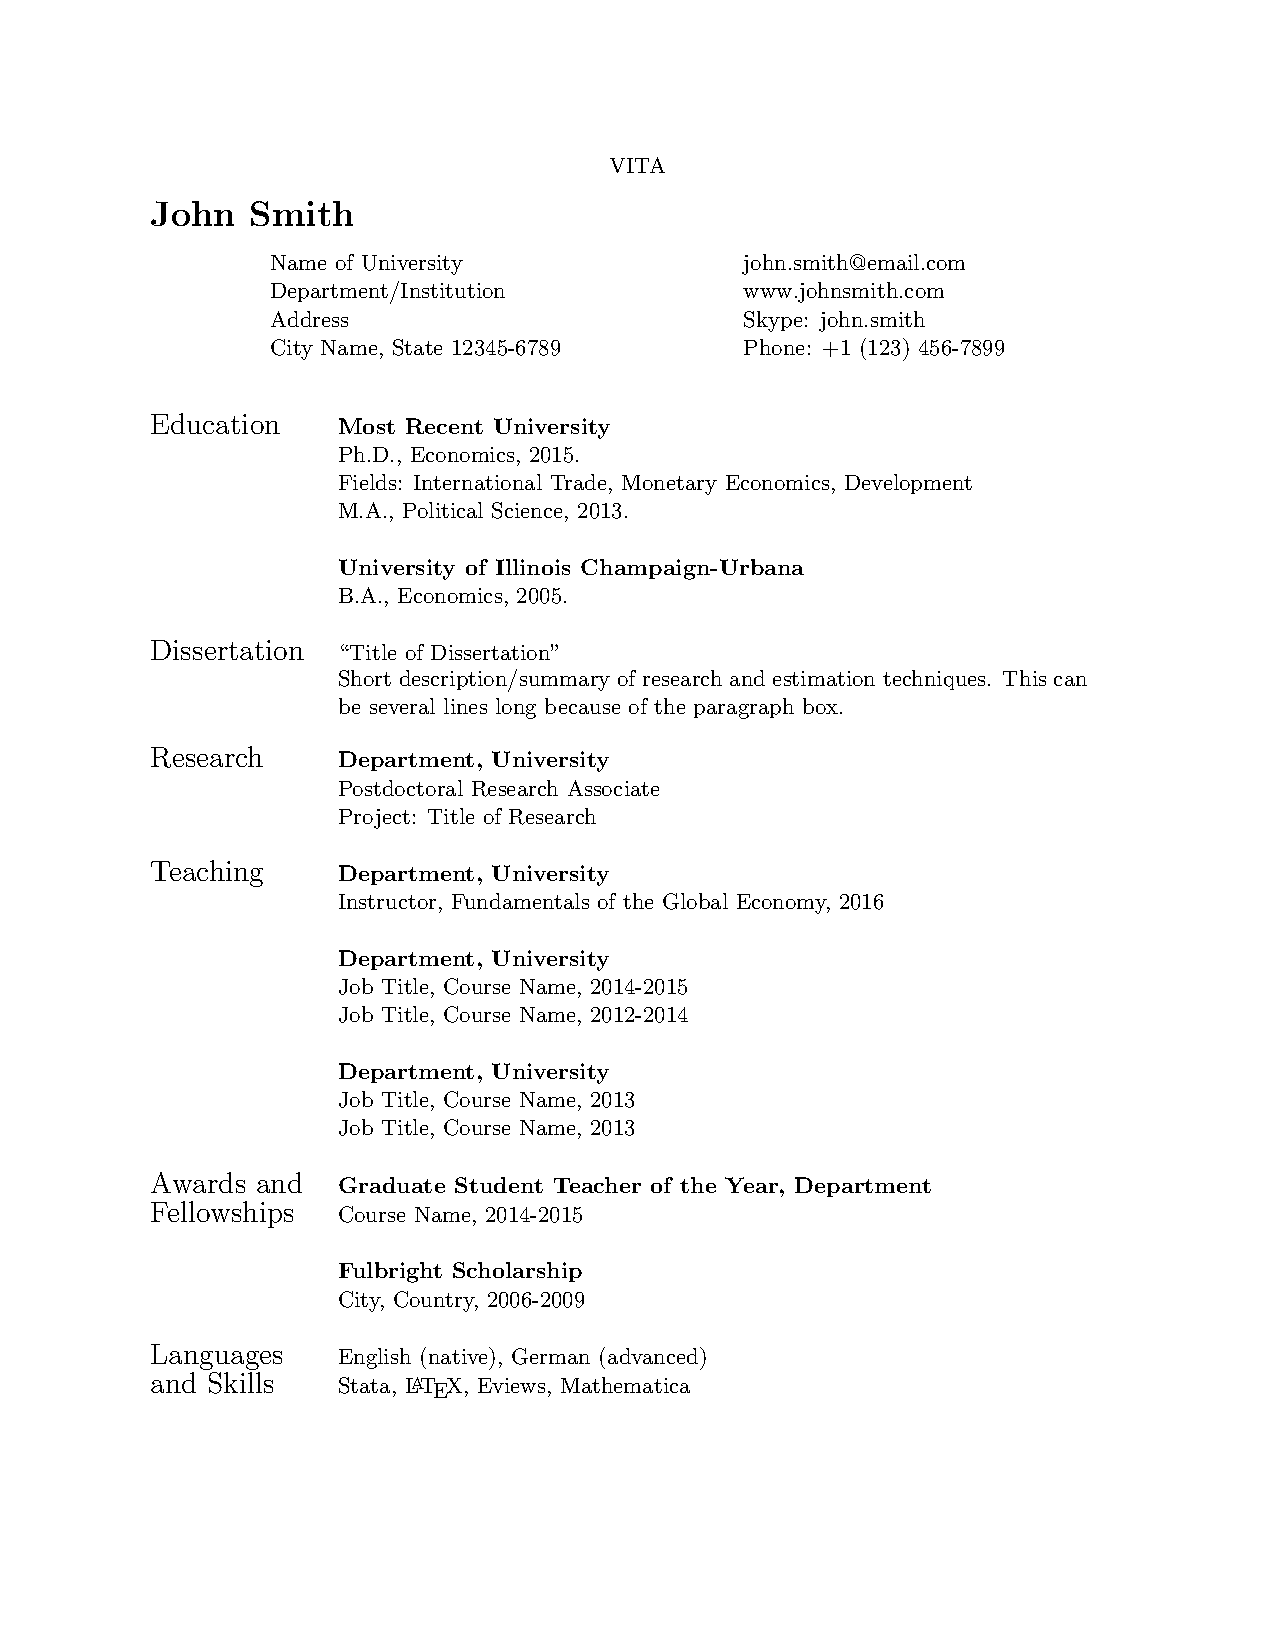
\includepdf[pagecommand={\thispagestyle{plain}}]{cv.pdf}
	% You will need to open the cv.tex file and edit the contents. Next, compile the document. That creates the pdf file that is referenced in the command above. Then, your cv will appear with page numbers in the correct spot in your document.

\end{document}
